\documentclass{article}
\usepackage[utf8]{inputenc}
\usepackage{natbib}
\usepackage{graphicx}
\usepackage{amsmath}
\usepackage{amssymb}

\title{Notes on paper Tesis UFRO}
\author{Juan P. Gil }
\date{May 2018}


\begin{document}

\maketitle

\begin{abstract}
Notes towards make the article to be sent as part of the Master Degree.
\end{abstract}


% \begin{figure}[h!]
% \centering
% 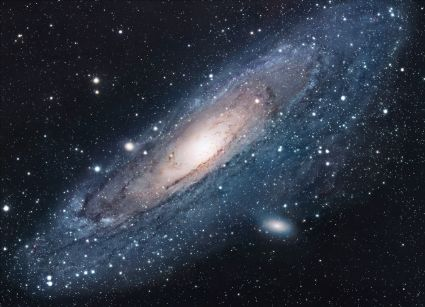
\includegraphics[scale=1.7]{universe}
% \caption{The Universe}
% \label{fig:universe}
% \end{figure}


\section{Introduction}

General information regarding the log analysis.
Hardware and software at observatory facilities.


Proposal: generate a set of features from event logs to describe time intervals.

Goals of the work: to detect outliers.

framework of the problem, state of the art, uses of the applied technique
classical approaches, paper proposal. Goals of the study
Organization of the rest of the paper


\section{Data Source}

La idea principal aqui es mostrar como filtre los logs para extraer los casos. Mas adelante centrare los analisis en 1) Casos particulares, y 2) Alguna mezcla entre casos.

\subsection{Logs at ALMA}

\subsection{Log Recollection}

log rate generation


\subsection{Use Cases}
Events generated by antennas

how to extract the value to study

-- train and test sets



\section{Method}

\subsection{Definitions}

Intuitively, an event is an entry in the log defined by its timestamp and the activity performed. While in practice there are valuable information coded in activities, for this analysis they are considered as an indivisible entity. The log is filtered in individual cases belonging to the same high level use case, a distinction made a priori by some domain specialist.

Given a finite set of \emph{activities} $A \neq \o$, we define an \emph{event} as the ordered pair 

\begin{equation}
\begin{split}
    e = (\tau, a) \in \mathbb{R} \times A
\end{split}
\end{equation}

where $\tau$ is referred as the \emph{event time}. 

A \emph{case} $C$ of size $n$ is a finite ordered sequence of events denoted by:

\begin{equation}
\begin{split}
    C & = (\tau_1,a_1)(\tau_2,a_2)  \dots (\tau_n,a_n) \\ 
      & = e_1 e_2 \dots e_n \\
      & = (e_i)_{i \leq n} \\
      & = ( (\tau_i, a_i) )_{i \leq n}
\end{split}
\end{equation}

with $n > 0$ and $\tau_j \geq \tau_i\ \forall\ i > j$. The size of $C$ will be denoted as $|C| = n$

The $Trace(C)$ is the sequence of activities for a given case: 

\begin{equation}
    Trace(C) = a_1 a_2 \dots a_n = (a_i)_{i \leq n}
\end{equation}

such that $\forall e_i=(\tau_i, a_i) \in C, Trace(C)_i = a_i$. Note that the trace preserves the order of activities, and that $|Trace(C)| = |C|$

Finally a \emph{Log} $L$ of size $M$ is the finite set of cases 

\begin{equation}
    L = \{C^1, \dots, C^M\}
\end{equation}

Table \ref{table:case_example} shows an example of a case with 14 events where $e_1 = (0, A), e_2 = (3, B), ... , e_{14} = (65, Z)$.


\subsection{Delay Measurement}

Measure the times between different pairs of events can lead to a too much operations given that the number of possible pairs (allowing activiy repetition) is 

$$| \{ e_1e_1, e_1e_2, ... , e_{n-1}e_n, e_ne_n \} | = |C|^2$$

To avoid this number some assumptions are made.

\emph{Assumption 1}: Start/End events must be different. 

\emph{Assumption 2}: Only pairs of events with same apparition frequency in the trace are considered. The log is generated by an implicit process, then it is reasonable to expect pairs of event that can be assumed as Start/End points and the idea is to measure the time intervals (delays) between them. Besides, a serial process can be considered as a combinations of Start/End points of an abstract process. Under ideal scenarios, where the process is executed without errors, these Start/End points appears the same amount of times inside a given case. 

\emph{Assumption 3:} The order of Start/End is defined by first appearance in trace. Therefore, if an interval between $(c_ic_j)$ is measured, then $(c_jc_i)$ is not.

The following definitions are focused to work with events inside a case, then mixing up with other cases assuming that the same activities has same behavior among all the cases in a log.

Given a case $C$ over a set of activities $A$, for every $s \in A$ the frequency $f_C(s)$ is defined as the number of instances that $s$ appears in the trace:

\begin{equation*}
    f_C(s)=|\{ (\tau_i, a_i)\ |\ a_i = s; \forall a_i \in Trace(C)  \}| 
\end{equation*}

Two activities $a_i, a_j \in Trace(C)$ are said to be \emph{near} if 

$$a_k \neq a_i; a_k \neq a_j \quad \forall i < k < j$$

that is, there are no instances of $a_i, a_j$ between them.

The order of apparition of an activity is defined as follow. Given a case $C$ such that $Trace(C) = a_1 \dots a_{i-1} a_i \dots a_j \dots$, the relation between activities $a_i \gtrdot_C a_j$, denoted as $a_j$ is called a \emph{successor} of $a_i$, is defined as

\begin{equation}
    a_i \gtrdot_C a_j \iff a_j \neq a_k; 1 \leq k \leq i 
\end{equation}

Given two events $e_i=(\tau_i, a_i), e_j=(\tau_j, a_j)$ belonging a case $C$, if $a_i$ and $a_j$ are near and $a_i \gtrdot_C a_j$, then $a_j$ is a \emph{nearest succesor} of $a_i$ at time $\tau_j$, and it is denoted as

\begin{equation}
    a_i \doteqdot_C a_j(\tau_j)
\end{equation}

Some properties emerges immediately from the definitions: an activity can have no successors, for example in $Trace(C)=a$ (single activity). The relation $a_i \gtrdot_C a_j$ is asymmetrical, that is, for a given case $C$ if $a_i \gtrdot_C a_j$ then $a_i$ is not a successor of $a_j$. The successor $a_i \gtrdot_C a_j$ don't have unicity because it could exists $a_i \gtrdot_C a_k$ with $a_j \neq a_k$. In contrast, if $a_i, a_j, \tau_j$ exists such that $a_i \doteqdot_C a_j(\tau_j)$, then $(\tau_j, a_j)$ is unique. The relation $a_i \doteqdot_C a_j(\tau_j)$ implies $a_i \gtrdot_C a_j$ whose definition implies $a_i \neq a_j$, then there are no successor nor nearest succesor of itself:

\begin{equation}
\begin{split}
              a_i \gtrdot_C a_j & \Rightarrow a_i \neq a_j \\
    a_i \doteqdot_C a_j(\tau_j) & \Rightarrow a_i \neq a_j
\end{split}
\end{equation}

Finally, we restrict the possible pairs of events over which we study the delays. A \emph{pairwise comparable} $\mathcal{P}_C$ set for a case $C$ is the set of nearest successors with same frequency, defined as

\begin{equation} \label{eq:pairwaise_comparable}
\begin{split}
     \mathcal{P}_C \subset A \times \mathbb{R} \times A \times \mathbb{R} \\
     ((a_i, \tau_i), (a_j,\tau_j)) \in \mathcal{P}_C \iff & (a_i, \tau_i) \in C \\
     & (a_j,\tau_j) \in C \\
     & a_i \doteqdot_C a_j(\tau_j) \\
     & f_C(a_i) = f_C(a_j)
\end{split}
\end{equation}


% Such pair $e_ie_j$ is said to be \emph{comparable}. It is denoted as

Now let's define the time interval elapsed between events, also referred as delay. The \emph{delay at time} $\tau_j$ between two pairwise comparable events $e_i=(\tau_i, a_i)$, $e_j=(\tau_j, a_j)$ of a case $C$ is defined as:

\begin{equation} \label{eq:comparable_delays}
\begin{split}
    \delta_C & : \mathcal{P}_C \rightarrow \mathbb{R} \\
    \delta_C( e_i, e_j ) & = \tau_j - \tau_i \\
    \delta_C( (\tau_i,a_i), (\tau_j, a_j) ) & = \tau_j - \tau_i 
\end{split}
\end{equation}

By definition of $C$ and the properties of $\doteqdot_C$, it is ensured that $\delta_C \geq 0$, however there are pairs $( e_i, e_j )$ where $\delta_C$ is not defined, for example the inverse pair $(e_j, e_i)$ for a defined delay $\delta_C( e_i, e_j )$. 

If we are restricted to a single case $C$, the function $\delta_C( (\tau_i,a_i), (\tau_j, a_j) )$ can be abbreviated as $\delta_{a_ia_j}(\tau_j)$. The nearest successor condition ensures that only nearest events are being measured to avoid ambiguity, as $\delta_{ab}(\tau)$ in $Trace(C)=ababababab \dots$ for some $\tau$. 

An example of delays between comparable pairs is shown in table \ref{table:case_example}.

\begin{table}[h]
\centering
\begin{tabular}{||c c||c c||c c c||c c||c||} 
 \hline
 $\tau$ & Activity & \multicolumn{2}{|c||}{Freq=1} & \multicolumn{3}{|c||}{Freq=2} & \multicolumn{2}{|c||}{Freq=3} & $\delta_{a_i a_j}(\tau_j)=\tau_j - \tau_i$ \\
 \hline\hline
 0  & A & A &   &   &   &   &   &   & \\
 \hline
 3  & B &   &   &   &   &   & B &   & \\
 \hline
 10 & C &   &   &   &   &   &   & C & $\delta_{BC}(10)=7$ \\
 \hline
 15 & B &   &   &   &   &   & B &   & \\
 \hline
 20 & D &   &   & D &   &   &   &   & \\
 \hline
 25 & C &   &   &   &   &   &   & C & $\delta_{BC}(25)=10$ \\
 \hline
 30 & E &   &   &   & E &   &   &   & \\
 \hline
 35 & B &   &   &   &   &   & B &   & \\
 \hline
 40 & F &   &   &   &   & F &   &   & $\delta_{EF}(40)=10, \delta_{DF}(40)=20$ \\
 \hline
 45 & C &   &   &   &   &   &   & C & $\delta_{BC}(45)=5$ \\
 \hline
 49 & E &   &   &   & E &   &   &   & \\
 \hline
 55 & D &   &   & D &   &   &   &   & \\
 \hline
 60 & F &   &   &   &   & F &   &   & $\delta_{EF}(60)=11, \delta_{DF}(60)=5$ \\
 \hline
 65 & Z &   & Z &   &   &   &   &   & $\delta_{AZ}(65)=65$ \\
 \hline
\end{tabular}
\caption{Example of a case with $A = \{ A, B, C, D, E, F, Z \}$. The activities where grouped by its frequency in $Trace(C)$ and the $\delta_{ab}(\tau)$ function was calculated over comparable pairs. The combined delays are $\Delta(A,Z)=(65)$, $\Delta(B,C)=(7,10,5)$, $\Delta(E,F)=(10,11)$, $\Delta(DF)=(20,5)$}.
\label{table:case_example}
\end{table}

Equation \ref{eq:comparable_delays} defines a single point but we need a serie of such delays relating $a_i$ and $a_j$. Multiple approaches are now possible to combine the delays. The simplest way is to merge all the delays of a comparable pair in a single vector, disregarding the order.

Let be $\Delta_C(a, b)$ a serie containing all delays for activities $a$, $b \in A$ in a case $C$

\begin{equation}
\begin{split}
    \Delta_C(a, b) & = \delta_{ab}(\tau_1) \delta_{ab}(\tau_2) \dots \delta_{ab}(\tau_N) \\
                   & = \Big( \delta_C\big( (\tau_i,a), (\tau_j, b) \big) \Big)_{\big( (\tau_i,a), (\tau_j, b) \big) \in \mathcal{P}_C}
\end{split}
\end{equation}

And $\Delta(a, b)$ the union of all $\Delta_C(a, b)$ in a single vector

\begin{equation} \label{eq:all_delays}
    \Delta_(a, b) = \bigcup_{i} \Delta_{C_i}(a, b) \quad \forall C_i \in L
\end{equation}

Such $\Delta(a, b)$ will be subject of statistical analysis in order to characterize the comparable pair $(a,b)$.


\subsection{Delay Analysis}


---

The Serial Case

Correlations. 

Introducing Parallelism

Random Traces

\subsection{Implementation of the Algorithm}

Order, steps, performance


\section{Simulated Event Logs}

Parameters: activities, serial to parallel, log size

comparison with other methods

\subsection{Synthetic Generator}



\section{Case Study: Antenna operation}

results by the method
domain expert analysis
parameter calibration

\section{Conclusion}

``I always thought something was fundamentally wrong with the universe'' \citep{adams1995hitchhiker}


\bibliographystyle{plain}
\bibliography{references}
\end{document}
